\chapter{Methodology}

This chapter presents the methodology used to model and predict short-horizon \ac{HDV} maneuvers in highway traffic. 
Starting from raw vehicle trajectories in the highD dataset, the proposed pipeline constructs a vehicle-centric representation, 
derives interaction and risk-related features, aggregates them over short temporal windows, and uses the resulting observation sequences 
to train and evaluate a hierarchical \ac{DBN}.

\par The target of prediction is a discrete maneuver class rather than an exact continuous future trajectory. 
The model therefore focuses on high-level action categories such as acceleration, braking, lane changes, and stable following.
To support this prediction task, the observation space combines ego-motion variables with contextual information from 
surrounding vehicles and safety-related quantities that describe the current traffic situation.

\par The remainder of this chapter describes the overall framework, the dataset used in this work, the preprocessing and 
feature-engineering pipeline, the window-based observation representation, the proposed \ac{DBN} structure, 
and the training and inference procedure. It also introduces the prediction-explanation procedure used to provide a local 
interpretation of the inferred latent state and maneuver prediction.


\section{Proposed Framework}

The proposed framework converts raw highD trajectory data into structured temporal observations for maneuver prediction.
Its main stages are data preparation, feature extraction, temporal window aggregation, \ac{DBN} training, and inference.

\par The pipeline starts from frame-level trajectories and transforms them into a consistent vehicle-centric representation.
Based on the ego vehicle and its local traffic environment, additional features are derived to capture interaction context, 
lane-related information, and risk-related properties such as \ac{THW} and \ac{TTC}.
These steps provide a compact description of the current driving situation beyond the ego vehicle alone.

\par Since maneuver prediction depends on recent temporal context, the frame-level signals are not used directly as isolated observations.
Instead, they are aggregated over short sliding windows to form a window-based sequence representation. 
Each window summarizes recent motion and interaction patterns and serves as one observation for the probabilistic model.

\par The prediction model is formulated as a hierarchical \ac{DBN} with two discrete latent variables: a driving-style state and an action state. 
This structure enables the model to represent both broader traffic-regime differences and maneuver-specific behavioral variation. 
The engineered window features are linked to the latent states through the emission model, while the temporal evolution of behavior is modeled through the state transitions.

\par Model parameters are estimated from the training data using an \ac{EM}-based learning procedure. 
To avoid information leakage, the windowized sequences are split at vehicle level into training, validation, and test sets before model fitting. 
After training, the learned model is used to infer the posterior distribution over latent states for new observation sequences and to predict the current maneuver distribution.

\par An overview of the complete framework is shown in Figure~\ref{fig:proposed_framework}. 
The individual stages are described in detail in the following sections.

\begin{figure}[htbp]
    \centering
    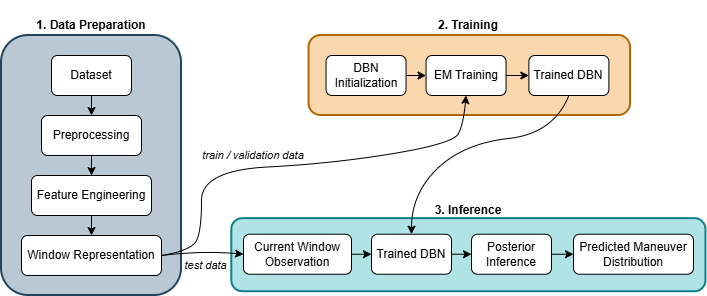
\includegraphics[width=0.95\linewidth]{images/Framework.drawio.png}
    \caption[Overview of the proposed framework]{Overview of the proposed framework}
    \label{fig:proposed_framework}
\end{figure}

\section{Dataset}

This thesis uses the highD dataset \cite{krajewski2018highddatasetdronedataset}, a naturalistic highway-traffic dataset recorded from drone videos on German highways.
Its aerial perspective provides frame-level trajectories together with surrounding-vehicle information, making it well suited for the analysis of human driving behavior in highway scenarios.

\par The full highD dataset contains 60 recordings collected at several highway locations. 
In this work, only the first 25 recordings with three lanes in each driving direction are used. 
This restriction provides a more uniform road geometry and traffic setting across the selected subset, which supports more consistent behavior modeling.
Figure~\ref{fig:highd_scene_example} shows an example traffic scene from the selected subset and illustrates the multi-lane highway layout together with the surrounding-vehicle 
context available for each target vehicle.
\begin{figure}[htbp]
    \centering
    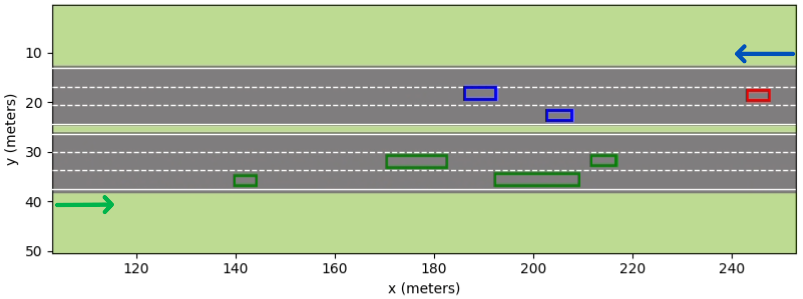
\includegraphics[width=0.9\linewidth]{images/dataset_illustration.png}
    \caption[Example traffic scene from a selected highD subset]{Example traffic scene from a selected highD subset. The red box denotes the ego vehicle, while the blue and green boxes represent other vehicles traveling in the two opposite driving directions.}
    \label{fig:highd_scene_example}
\end{figure}

\par For each vehicle, highD provides frame-level trajectory variables such as longitudinal and lateral position, velocity, and acceleration.
It also includes lane-related information, driving-direction labels, and identifiers for neighboring vehicles in relevant surrounding positions.
In addition, the dataset provides traffic-safety indicators such as \ac{TTC} and \ac{THW}, which support the construction of interaction and risk-related features. 
These signals form the basis for the preprocessing and feature-engineering pipeline described in the next sections.

\par For the selected subset, 50,543 vehicle trajectories are available after loading the chosen recordings. 
With a window length of \(W=50\) frames, 50,455 trajectories satisfy \(T \geq W\), while only 88 are shorter than the required window length.  
The trajectory lengths are well suited for temporal modeling, with a 10th percentile of 280 frames, a median of 349 frames, and a 90th percentile of 466 frames.  
This indicates that the selected subset is sufficiently large and temporally rich for constructing window-based observation sequences.

\section{Data Preparation and Preprocessing}

\subsection{Preprocessing Pipeline}

The raw highD files are first merged into a unified per-frame representation that combines trajectory data with vehicle-level and recording-level metadata. 
Since the dataset contains multiple recordings, each trajectory is uniquely identified by the pair (recording\_id, vehicle\_id). In addition, 
vehicle-center coordinates are computed from the original bounding-box positions in order to provide a consistent geometric reference for the subsequent 
construction of context features. 

\par As the selected recordings contain traffic moving in two opposite roadway directions, the raw image-based coordinates cannot be used directly 
as a homogeneous representation.
A vehicle-centric normalization step is therefore applied using the driving-direction label. 
This transformation adjusts the sign convention of the longitudinal and lateral motion variables such that forward and lateral motions are represented consistently across both traffic directions. 
As a result, the learned model receives a unified representation in which the same maneuver follows the same sign convention regardless of the original roadway direction.


\par At preprocessing stage, the available neighboring positions include the front, rear, left-front, left-side, left-rear, right-front, right-side, and right-rear slots. 
For each available neighbor, binary existence flags are created and relative kinematic quantities are derived in the form of relative longitudinal distance, relative lateral distance, relative longitudinal velocity, and relative lateral velocity. 
Missing neighbors remain explicitly marked through the corresponding existence indicators, while the relative features remain undefined when no matching neighbor state is available. 

\par In the final observation vector, only the subset shown in Figure~\ref{fig:neighbor_slots} is retained. 
This design focuses the model on the vehicles that most directly describe immediate car-following constraints in the current lane and the local traffic state of the adjacent lanes, 
while keeping the feature space compact and interpretable.
The omitted rear and rear-diagonal neighbors may also contain useful information, 
but they are excluded here as a simplifying design choice to limit feature dimensionality in the proposed \ac{DBN}.
\begin{figure}[htbp]
    \centering
    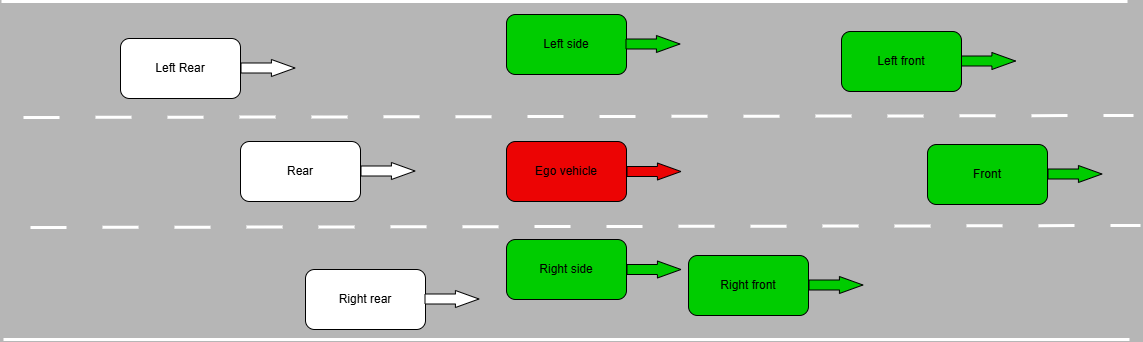
\includegraphics[width=0.9\linewidth]{images/neighbours.png}
    \caption[Selected neighbors considered in the observation]{Selected neighbors considered in the observation.}
    \label{fig:neighbor_slots}
\end{figure}

\par In addition to interaction features, the preprocessing step derives lane-related and risk-related quantities. 
Distances to the left and right lane boundaries are computed from the recording metadata and the ego-vehicle center position.
The lane-change indicator is obtained from changes in lane ID and represented as a ternary variable corresponding to lane change to left, no lane change, and lane change to right. 
The front-interaction safety signals provided by highD are mapped to the standardized variables \texttt{front\_thw} and \texttt{front\_ttc}. 
Furthermore, ego-vehicle jerk is computed from the frame-to-frame change in longitudinal and lateral acceleration.


\par Finally, the processed dataframe is reduced to the selected frame-level observation columns and metadata fields used in the subsequent sequence-construction stage. 
This produces a consistent per-frame representation that serves as the basis for feature aggregation and windowization.


\subsection{Data Analysis for Feature Design}

Before defining the final observation vector, an exploratory analysis of the highD varables was carried out to understand the statistical behaviour of the available signals 
and to identify features that are informative. The analysis focused mainly on kinematic variables, namely longitudinal and lateral acceleration 
$(a_x, a_y)$, longitudinal and lateral velocity $(v_x, v_y)$, and simple lane-change indicators. 


\begin{figure}[htbp]
    \centering

    \begin{subfigure}[t]{0.48\textwidth}
        \centering
        
\includegraphics[height=5cm]{images/ax__global.png}
        \caption{Longitudinal acceleration.}
        \label{fig:data_analysis_ax_global}
    \end{subfigure}
    \hfill
    \begin{subfigure}[t]{0.48\textwidth}
        \centering
        
\includegraphics[height=5cm]{images/ay__global.png}
        \caption{Lateral acceleration.}
        \label{fig:data_analysis_ay_global}
    \end{subfigure}

    \vspace{0.6em}

    \begin{subfigure}[t]{0.48\textwidth}
        \centering
        
\includegraphics[height=5cm]{images/vx__global.png}
        \caption{Longitudinal velocity.}
        \label{fig:data_analysis_vx_global}
    \end{subfigure}
    \hfill
    \begin{subfigure}[t]{0.48\textwidth}
        \centering
        
\includegraphics[height=5cm]{images/vy__global.png}
        \caption{Lateral velocity.}
        \label{fig:data_analysis_vy_global}
    \end{subfigure}
 
    \caption{Global distributions of the main kinematic variables.}
    \label{fig:data_analysis_kinematics_global}
\end{figure}


\par As shown in \autoref{fig:data_analysis_ax_global}, the distribution of $a_x$ is centred near zero but has visible tails on both sides, 
indicating that most frames correspond to near-steady motion, while stronger acceleration and braking occur less often. 
The longitudinal velocity distribution in \autoref{fig:data_analysis_vx_global} spans a broad range of values and exhibits a multimodal structure.
This is mainly caused by differences between vehicle classes, with trucks concentrated at lower speeds and cars occupying a wider and generally higher-speed range. 
These class-dependent differences show that raw continuous features can have different natural ranges depending on the vehicle type.  
For this reason, continuous variables are standardized before training, as described later in the training subsection.

\begin{figure}[!t]
    \centering

    \begin{subfigure}[t]{0.48\textwidth}
        \centering
        
\includegraphics[height=5cm]{images/std__ax__global.png}
        \caption{Longitudinal acceleration.}
        \label{fig:std_ax_global}
    \end{subfigure}
    \hfill
    \begin{subfigure}[t]{0.48\textwidth}
        \centering
        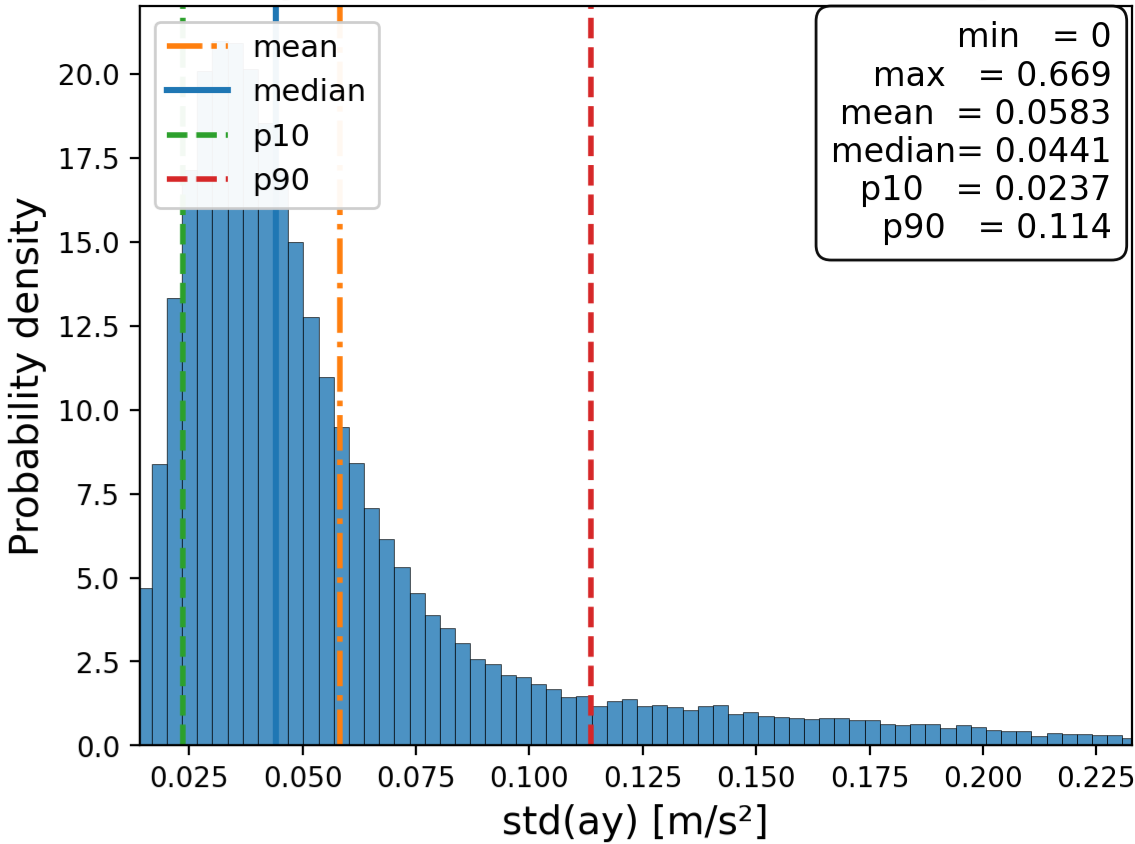
\includegraphics[height=5cm]{images/std__ay__global.png}
        \caption{Lateral acceleration.}
        \label{fig:std_ay_global}
    \end{subfigure}

    \vspace{0.6em}

    \begin{subfigure}[t]{0.48\textwidth}
        \centering
        
\includegraphics[height=5cm]{images/std__vx__global.png}
        \caption{Longitudinal velocity.}
        \label{fig:std_vx_global}
    \end{subfigure}
    \hfill
    \begin{subfigure}[t]{0.48\textwidth}
        \centering
        
\includegraphics[height=5cm]{images/std__vy__global.png}
        \caption{Lateral velocity.}
        \label{fig:std_vy_global}
    \end{subfigure}

    \caption{Global trajectory-level variability distributions of the main kinematic variables.}
    \label{fig:variability_global_kinematics}
\end{figure}

On the other hand, the lateral variables are much more concentrated around zero.  
In \autoref{fig:data_analysis_ay_global} and \autoref{fig:data_analysis_vy_global}, both $a_y$ and $v_y$ show sharp peaks near zero, 
which is expected because most vehicles remain within their lane for most of the time.
However, the non-zero tails still reflect lateral adjustments and lane-change-related motion. 
Together, these observations support the inclusion of both longitudinal and lateral kinematic variables, 
since the former describe speed adaptation and car-following behaviour, whereas the latter provide cues for lateral maneuvers.


\par In addition to the raw frame-level signals, the variability of each kinematic variable was also analysed at trajectory level. 
For each vehicle trajectory, the standard deviation of $a_x$, $a_y$, $v_x$, and $v_y$ was computed over time, producing one variability value per trajectory.  
Unlike the raw kinematic distributions, these plots do not describe the absolute values of the signals, but rather how strongly they 
fluctuate within individual trajectories.
The resulting distributions are shown in \autoref{fig:std_ax_global} to \autoref{fig:std_vy_global}. 

\par The variability analysis shows that longitudinal motion is generally more dynamic than lateral motion.
In \autoref{fig:std_ax_global} and \autoref{fig:std_vx_global}, both $\mathrm{std}(a_x)$ and $\mathrm{std}(v_x)$ exhibit broader distributions with long right tails, 
indicating that some vehicles undergo substantial longitudinal speed and acceleration changes.
In contrast, \autoref{fig:std_ay_global} shows that $\mathrm{std}(a_y)$ remains concentrated at low values, which is consistent with lateral acceleration being 
close to zero except during lane changes.
A similar pattern appears in \autoref{fig:std_vy_global}, although the visible tail suggests that some trajectories contain stronger lateral motion. 
These results support the use of variability-related window features, since instantaneous values alone do not capture whether a trajectory is stable or dynamically changing over time.


\par The lane-change analysis further highlights an important property of the dataset.
As shown in \autoref{fig:lc_frame_distribution}, almost all frames belong to the lane-keeping class, while left and right lane changes occur only rarely. 
The same sparsity appears at trajectory level in \autoref{fig:lc_per_trajectory}, where most 
vehicles perform no lane change and only a small fraction perform one or more. 
This imbalance shows that lane-change events are very rare compared to straight driving. 
It also shows that the raw lane-change indicator alone is not sufficient as a learning signal, especially 
because in highD the lane change is marked only at the frame where the vehicle crosses the lane boundary.
This motivated the use of temporal aggregation together with contextual kinematic and interaction features.




\begin{figure}[htbp]
    \centering

    \begin{subfigure}[t]{0.48\textwidth}
        \centering
        
\includegraphics[height=4.95cm]{images/lane_change_frame_distribution.png}
        \caption{Raw lane-change indicator at frame level.}
        \label{fig:lc_frame_distribution}
    \end{subfigure}
    \hfill
    \begin{subfigure}[t]{0.48\textwidth}
        \centering
        
\includegraphics[height=4.8cm]{images/lane_changes_per_trajectory.png}
        \caption{Number of lane changes observed per trajectory.}
        \label{fig:lc_per_trajectory}
    \end{subfigure}

    \caption{Lane-change sparsity analysis in the highD data.}
    \label{fig:lane_change_analysis}
\end{figure}

\par Overall, the data analysis led to three main conclusions. 
First, longitudinal and lateral kinematics provide complementary information for maneuver prediction. 
Second, trajectory-level variability contains useful information beyond instantaneous frame values. 
Third, feature scale and class-dependent distribution differences must be handled carefully during preprocessing. 
These findings directly guided the feature engineering, where the raw signals were transformed 
into the final observation features for the proposed \ac{DBN} model.
\FloatBarrier



\subsection{Feature Engineering}
Based on the preprocessing steps described above, the final frame-level observation was defined as the compact feature set listed in Table~\ref{tab:frame_features}. 
The selected variables describe ego motion, lane-change evidence, lane geometry, local interaction context, and front-interaction risk. 
This frame-level representation serves as the basis for the subsequent window-based observation model.


\begin{table}[htb]
    \centering
    \small
    \caption{Frame-level feature groups used in the preprocessing pipeline}
    \label{tab:frame_features}
    \begin{tabular}{p{2.9cm} p{4.8cm} p{4.6cm}}
        \toprule
        \textbf{Feature group} & \textbf{Variables} & \textbf{Purpose} \\
        \midrule
        Ego kinematics & \texttt{vx}, \texttt{vy}, \texttt{ax}, \texttt{ay}, \texttt{jerk\_x}, \texttt{jerk\_y} & Describe recent ego motion and control variation \\
        Lane-change evidence & \texttt{lc} & Encode left / none / right lane-change evidence \\
        Lane geometry & \texttt{d\_left\_lane}, \texttt{d\_right\_lane} & Represent lateral position within the current lane \\
        Front risk & \texttt{front\_thw}, \texttt{front\_ttc} & Describe front-interaction criticality \\
        Neighbor existence & Existence indicators for the selected front and adjacent-lane neighbor slots & Indicate whether relevant surrounding vehicles are present \\
        Relative interaction & For each selected neighbor slot: \texttt{dx}, \texttt{dy}, \texttt{dvx}, \texttt{dvy} & Capture relative position and motion with respect to surrounding traffic \\
        \bottomrule
    \end{tabular}
\end{table}


\subsection{Window-Based Representation}

The proposed \ac{DBN} operates on short temporal windows rather than on individual frames. 
Each vehicle trajectory is therefore converted into a sequence of overlapping windows, as illustrated in \autoref{fig:window_based_representation}.
This allows the model to use recent motion history and interaction context instead of relying only on instantaneous frame values.

\par Let $W$ denote the window length and $S$ the stride between consecutive windows. 
In this work, $W=50$ frames and $S=10$ frames are used. 
Since highD is recorded at 25\,Hz, each window covers approximately 2\,s of history, while consecutive windows start 0.4\,s apart. 
Thus, for a trajectory of length $T$ frames, overlapping windows are extracted every $S$ frames as long as $T \geq W$. 
Each resulting observation summarizes the selected features over one interval of $W$ consecutive frames.

\begin{figure}[htbp]
    \centering
    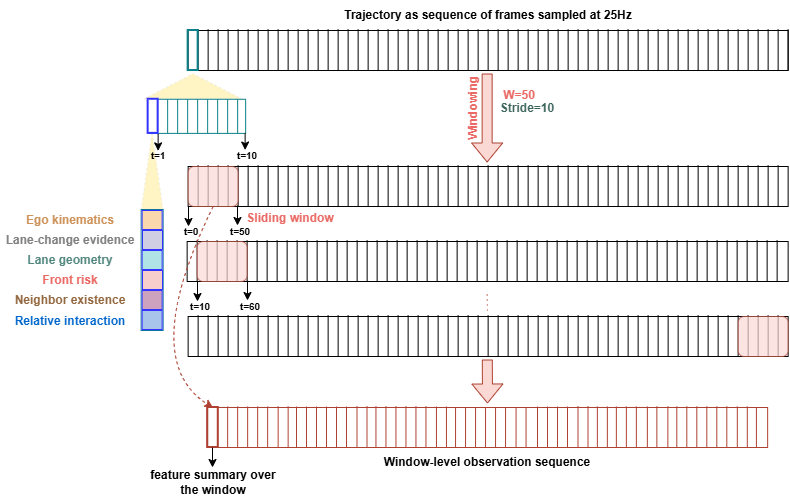
\includegraphics[width=0.95\linewidth]{images/windowize.png}
    \caption{Illustration of the sliding-window representation used in this work.}
    \label{fig:window_based_representation}
\end{figure}

\par Each window is converted into a single observation vector by aggregating the frame-level signals over the corresponding window interval. 
Depending on the variable, the aggregation uses the most recent value, a minimum over the window, a temporal slope, sign-based fractions, percentile-based summaries, 
binary event indicators, or fractions of valid or available frames. For neighbor-dependent variables, the summaries are computed only when the corresponding neighbor is present.
The complete list of window-level features used in the final observation vector is provided in Appendix~\ref{appendix:window_features}.
The resulting sequence of window-level observations forms the input to the proposed \ac{DBN} during both training and inference.




\section{Proposed DBN Model}
The proposed model represents driver behavior through two discrete latent variables: a style state $S_t$ and an action state $A_t$. 
The style state captures a broader driving regime, while the action state represents the maneuver at the current time step. 
The observation vector $O_t$ corresponds to the window-level features described in the previous section.

\subsection{Latent State Structure}
Rather than using a single latent variable, the model uses a factorized latent representation. 
As shown in \autoref{fig:proposed_dbn_structure}, the style state evolves over time as its own Markov chain, whereas the action state depends on both 
the previous action and the current style state. 
This structure allows the model to separate slower regime-level dynamics from faster maneuver-level changes.
\begin{figure}[htbp]
    \centering
    \begin{tikzpicture}[
    node distance=1.8cm and 1.8cm,
    >=Stealth,
    latent/.style={draw, circle, minimum size=9mm, inner sep=0pt, align=center}
]

\node[latent] (Sprev) {$S_{t-1}$};
\node[latent, right=of Sprev] (St) {$S_t$};
\node[latent, right=of St] (Snext) {$S_{t+1}$};

\node[latent, below=1.5cm of Sprev] (Aprev) {$A_{t-1}$};
\node[latent, below=1.5cm of St] (At) {$A_t$};
\node[latent, below=1.5cm of Snext] (Anext) {$A_{t+1}$};

\draw[->] (Sprev) -- (St);
\draw[->] (St) -- (Snext);

\draw[->] (Sprev) -- (Aprev);
\draw[->] (St) -- (At);
\draw[->] (Snext) -- (Anext);

\draw[->] (Aprev) -- (At);
\draw[->] (At) -- (Anext);

\end{tikzpicture}
    \caption{Factorized latent structure of the proposed DBN.}
    \label{fig:proposed_dbn_structure}
\end{figure}

\subsection{Transition Model}
Let $S_t$ denote the latent style state and $A_t$ the latent action state at time step $t$. 
The initial distribution is modeled as
\begin{align}
p(S_0) &= \pi_{s_0}, \\
p(A_0 \mid S_0) &= \pi_{a_0 \mid s_0}.
\end{align}

For later time steps, the transition model is factorized as
\begin{align}
p(S_t \mid S_{t-1}) &= A_s[S_{t-1}, S_t],\\
p(A_t \mid A_{t-1}, S_t) &= A_a[S_t, A_{t-1}, A_t].
\end{align}

This factorization reflects the assumption that the style state evolves more gradually, 
while the current maneuver depends on both the recent maneuver history and the current driving regime. 


\subsection{Emission Model Variants}

At each time step, the latent pair $(S_t, A_t)$ generates the window-level observation vector $O_t$. 
Two alternative emission formulations are considered in this work, as illustrated in \autoref{fig:emission_variants}. 
Both use the same latent transition structure and differ only in how the observation likelihood is parameterized. 
In both cases, the observation vector is split into continuous and binary components. 
The continuous part is modeled with diagonal Gaussian distributions, while the binary part is modeled with Bernoulli distributions.

\begin{figure}[htbp]
    \centering
    \begin{subfigure}[t]{0.48\textwidth}
        \centering
        \begin{tikzpicture}[
    node distance=1.5cm and 1.8cm,
    >=Stealth,
    latent/.style={draw, circle, minimum size=9mm, inner sep=0pt, align=center},
    block/.style={draw, rounded corners=2pt, text width=3.3cm, minimum height=1.05cm, align=center},
    combine/.style={draw, rounded corners=2pt, text width=3.6cm, minimum height=1.05cm, align=center},
    obs/.style={draw, rectangle, minimum width=11mm, minimum height=8mm, align=center}
]

\node[latent] (S) {$S_t$};
\node[latent, right=3.4cm of S] (A) {$A_t$};

\node[block, below=1.5cm of S] (Es) {Style expert\\$p_s(o_t \mid s_t;\,\theta^{(s)}_{s_t})$};
\node[block, below=1.5cm of A] (Ea) {Action expert\\$p_a(o_t \mid a_t;\,\theta^{(a)}_{a_t})$};

\node[combine, below=1.8cm of $(Es)!0.5!(Ea)$] (C) {PoE combine\\$\big/ Z_{s_t,a_t}$};

\node[obs, below=1.5cm of C] (O) {$O_t$};

\draw[->] (S) -- (Es);
\draw[->] (A) -- (Ea);

\draw[->] (Es) -- (C);
\draw[->] (Ea) -- (C);

\draw[->] (C) -- (O);

\end{tikzpicture}
        \caption{Product-of-experts emission.}
        \label{fig:poe_emission}
    \end{subfigure}
    \hfill
    \begin{subfigure}[t]{0.48\textwidth}
        \centering
        \begin{tikzpicture}[
    node distance=1.5cm and 1.8cm,
    >=Stealth,
    latent/.style={draw, circle, minimum size=9mm, inner sep=0pt, align=center},
    block/.style={draw, rounded corners=2pt, text width=3.3cm, minimum height=1.05cm, align=center},
    combine/.style={draw, rounded corners=2pt, text width=3.6cm, minimum height=1.05cm, align=center},
    obs/.style={draw, rectangle, minimum width=11mm, minimum height=8mm, align=center}
]

\node[latent] (S) {$S_t$};
\node[latent, right=2.8cm of S] (A) {$A_t$};

\node[block, below=1.8cm of $(S)!0.5!(A)$] (E) {Joint emission\\$p(O_t \mid S_t,A_t)$};

\node[obs, below=1.5cm of E] (O) {$O_t$};

\draw[->] (S) -- (E);
\draw[->] (A) -- (E);
\draw[->] (E) -- (O);

\end{tikzpicture}
        \caption{Hierarchical emission.}
        \label{fig:hierarchical_emission}
    \end{subfigure}
    \caption{Emission model variants considered in the proposed DBN.}
    \label{fig:emission_variants}
\end{figure}

\subsubsection{Product-of-Experts Emission}
In the \ac{PoE} formulation, the observation likelihood is decomposed into two experts: one conditioned only on the style state and one 
conditioned only on the action state. 
Their contributions are combined multiplicatively and then normalized:
\begin{equation}
p(o_t \mid s_t, a_t) = \frac{p_s(o_t \mid s_t)\, p_a(o_t \mid a_t)}{Z_{s_t,a_t}},
\end{equation}
where $Z_{s_t,a_t}$ is the normalization term. 
This formulation allows the style state and the action state to contribute separately to the same observation vector.

\subsubsection{Hierarchical Emission}
In the hierarchical formulation, a single emission distribution is learned directly for each joint latent-state pair:
\begin{equation}
p(o_t \mid s_t, a_t)
=
\mathrm{Emission}(o_t; \theta_{s_t,a_t}).
\end{equation}
Here, the observation is modeled jointly for each combination of style and action. 
This gives the model more direct flexibility at the level of the joint latent state, at the cost of a larger number of emission parameters.


\par For both emission variants, the final output of the observation model is the log-likelihood tensor
\begin{equation}
\log p(O_t \mid S_t, A_t),
\end{equation}
evaluated for all combinations of style and action states at each time step. 
These values are then used together with the structured transition model during forward--backward inference and EM training. 
Thus, the proposed framework keeps the latent dynamics fixed at the DBN level, while allowing different observation models to be 
compared within the same inference and training pipeline.

\section{Training and Inference}
\subsection{Prediction Explanation}

\section{Semantic Interpretation of Latent States}